\documentclass{article}
\usepackage[T1]{fontenc}
\usepackage{lmodern}
\usepackage{graphicx}
\usepackage{amsmath,amssymb}
\usepackage[a4paper,margin=2cm]{geometry}
\usepackage[absolute,overlay]{textpos}
\setlength{\TPHorizModule}{1mm}
\setlength{\TPVertModule}{1mm}
\usepackage[indonesian]{babel}
\usepackage{hyperref}
\setlength{\emergencystretch}{2em}
% unit: Halaman 45

\begin{document}

% === Halaman 45 (python/native) ===

• Al-Kindi menulis buku tentang seni 

memecahkan kode, buku yang berjudul 

‘Risalah fi Istikhraj al-Mu'amma (Manuscript 

for the Deciphering Cryptographic Messages) 

• Al-Kindi menemukan frekuensi perulangan 

huruf di dalam Al-Quran. Teknik yang 

digunakan Al-Kindi kelak dinamakan analisis 

frekuensi.

• Yaitu teknik untuk memecahkan cipherteks 

berdasarkan frekuensi kemunculan karakter 

di dalam pesan

45

Halaman pertama buku Al-Kindi, 

Manuscript for the Deciphering Cryptographic

% deskripsi: gambar native xref 226
\noindent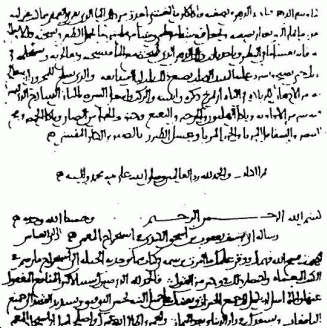
\includegraphics[width=0.85\textwidth]{../../images/python/page_045_img_01.png}

\end{document}
